\section{Evaluation}\label{sec:r2c:evaluation}
\subsection{System Configuration}\label{r2c:ss:eval-cfg} % about quarter of a page
% We performed the evaluation of the total overhead on four different machines.
We evaluate \rtwoc{} on four different machines.
Machine \propername{EPYC Rome} is equipped with an AMD EPYC Rome 7H12 CPU running at 3.2 GHz, 1TB DDR4 RAM running at 3200 MHz, and Debian 11.
Machine \propername{i9-9900K} is equipped with an Intel Core i9-9900K CPU running at 3.6 GHz, 64GB DDR4 RAM running at 2667 MHz, and Debian 11.
% Machine \propername{TR 3970X A} is equipped with an AMD Ryzen Threadripper 3970X CPU running at 3.7 GHz, 128GB DDR4 RAM running at 2400 MHz, and Debian 10.
Machine \propername{TR 3970X} is equipped with an AMD Ryzen Threadripper 3970X CPU running at 3.7 GHz, 128GB DDR4 RAM running at 2400 MHz, and Debian 10.
Machine \propername{Xeon} is equipped with an Intel Xeon Platinum 8358 CPU running at 2.60GHz, 256GB DDR4 RAM running at 3200 MHz, and Debian 11.

On each machine we used the bundled GCC and gold linker version to compile LLVM.
Our LLVM modifications are based on LLVM 11, and we compiled the benchmarks against the bundled \propername{glibc} and \propername{libstdc\plusplus} versions.
%    For \propername{musl} we used version 1.2.2 and the \propername{libc\plusplus} included with LLVM 11.

\subsection{Performance}\label{r2c:ss:perf}

To evaluate the performance impact of \rtwoc, we built and ran the SPEC CPU 2017 benchmark suite using our \rtwoc{} compiler.
The SPEC CPU 2017 suite is a collection of CPU-intensive C and \cpp benchmark programs.
%% We included the floating point benchmark suite to enable direct comparison with prior work \cite{vanderKouwe2019}.
To allow for direct comparison with prior work, we included the floating point benchmarks~\cite{vanderKouwe2019}.

We compiled all benchmarks with the \code{-O3} optimization level and link-time optimization---LLVM's ThinLTO model in our case---enabled.
As LLVM does not yet support the compilation of \propername{glibc}, we compiled the benchmarks against the unprotected system version of \propername{glibc} and \propername{libstdc\plusplus}.
To measure the worst-case overhead, we also enabled \glspl{BTRA} for call sites to unprotected code (see \cref{r2c:ss:limitations-coverage}).
For the evaluation of full \rtwoc{} we took the median execution time of 20 runs.
For the analysis of \rtwoc{}'s components we used \propername{EPYC Rome} and took the median execution time of 12 runs.
%\rtwoc{} inserts between one and five traps into each function prolog and each pair of \btra AVX setup instructions contains one to three NOPs (see \cref{r2c:ss:strengthening}).
Since the location of return addresses and the distribution of \glspl{heapbt} is random, we recompiled the benchmarks with a different seed for each of the executions.
To guarantee a fair comparison, we compiled the baseline with the same compiler version and flags but with \rtwoc disabled.

For the webserver benchmarks, we used \propername{wrk} as client and \propername{nginx} version 1.14.2 and \propername{Apache} version 2.4.54, serving 64-byte pages.
We split the CPU cores between \propername{wrk} and the webserver and gradually increased the number of concurrent connections until the CPU was fully saturated.
We compared the median throughput of five runs at the previously determined saturation connection count.
%Even when testing on the same host, however, we could not fully saturate the CPU, regardless of the number of connections\footnote{We tested up to 65536 connections and although the throughput started decreasing, the CPU saturation never exceeded 80\%}.

%To determine the incurred memory overhead for the SPEC benchmarks we recorded that maximum resident-set size of the benchmark processes.
%For the webservers we recorded the resident-set size of the parent webserver process in regular intervals and calculated the median.


%    To asses the performance impact of protecting the standard library we also built the benchmarks against a fully protected \propername{musl} libc and LLVM's \propername{libc\plusplus}.
%    Clang/LLVM currently does not compile the \propername{glibc} library, which is why we chose \propername{musl} and \propername{libc\plusplus} instead.
%    Since 2 of the 9 benchmarks in the benchmark suite are incompatible with \propername{musl}\footnote{The benchmarks \propername{perlbench} and \propername{gcc} are not compatible.}
%    and to ensure comparability with prior work, we report only the results of the \propername{glibc} based benchmarks here.
%    The performance results of the benchmarks compiled with the \musllib toolchain can be found in~\cref{apx:additional-benchmarks}.

\subsubsection{\glspl{BTRA}}\label{r2c:sss:eval-btra}
We evaluated the overhead of \glspl{BTRA} with the \code{push} setup and with our optimized AVX2 setup sequence respectively.
To isolate the overhead of \glspl{BTRA}, we disabled other diversification measures.
We configured \rtwoc{} to instrument each call site with a total of 10 \glspl{BTRA} and between 1 and 9 NOPs (see \cref{r2c:ss:strengthening}).

For the \code{push} setup, 10 \glspl{BTRA} mean that \rtwoc{} inserts up to 12 push instructions per call site: 11 for the \glspl{BTRA}, one for the return address, and one to keep the stack aligned (see \cref{r2c:ss:impl-btras}).
\cref{r2c:fig:perf-components} shows that the geometric mean overhead of this configuration is 6\%, but the outlier \propername{omnetpp} has an overhead of 21\%.


\begin{figure}[t]
    \centering
    \begingroup
    \pgfplotsset{
        every axis/.append style={
            yticklabel style={font=\propernamedecl\footnotesize},
            execute at begin axis={
                \pgfplotsset{
                    width=\textwidth,
                    height=0.8\linewidth}
            },
        },
    }
    \resizebox{\textwidth}{!}{% This file was created with matplot2tikz v0.4.2.
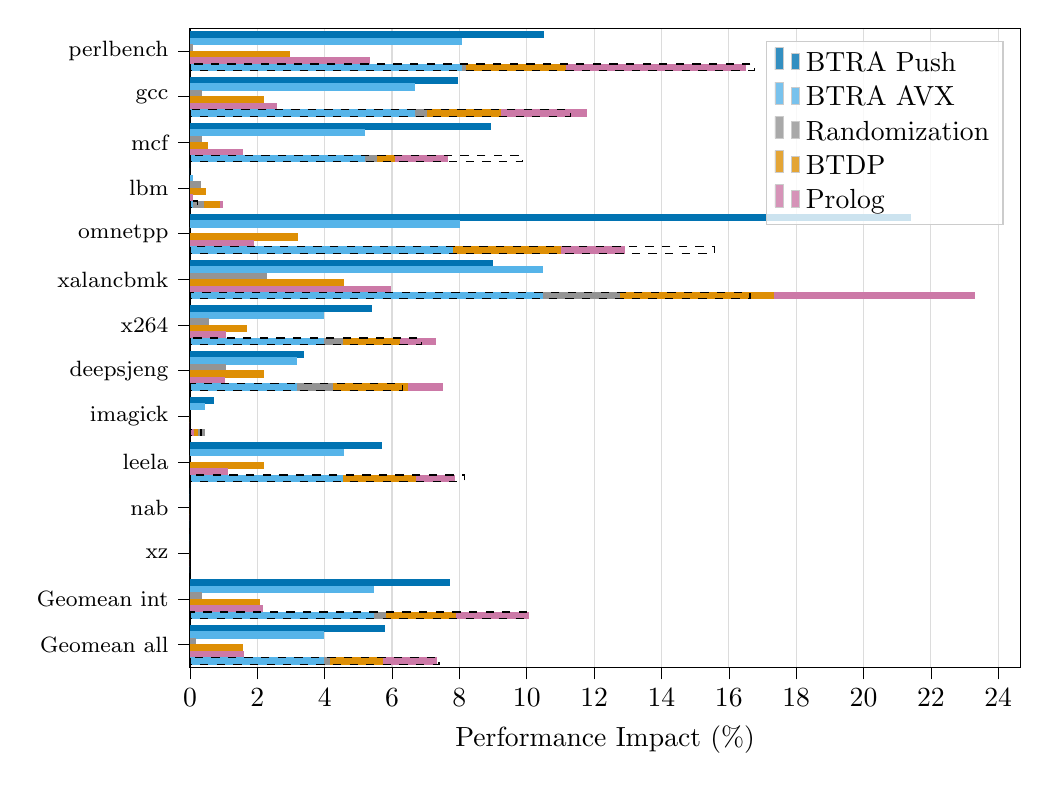
\begin{tikzpicture}

\definecolor{cornflowerblue86180233}{RGB}{86,180,233}
\definecolor{darkcyan1115178}{RGB}{1,115,178}
\definecolor{darkgray176}{RGB}{176,176,176}
\definecolor{darkorange2221435}{RGB}{222,143,5}
\definecolor{gainsboro}{RGB}{220,220,220}
\definecolor{lightgray204}{RGB}{204,204,204}
\definecolor{lightslategray148}{RGB}{148,148,148}
\definecolor{palevioletred204121167}{RGB}{204,121,167}

\begin{axis}[
legend cell align={left},
legend style={fill opacity=0.8, draw opacity=1, text opacity=1, draw=lightgray204},
tick align=outside,
tick pos=left,
x grid style={gainsboro},
xlabel={Performance Impact (\%)},
xmajorgrids,
xmin=0, xmax=24.6524209115605,
xminorgrids,
xtick style={color=black},
y dir=reverse,
y grid style={darkgray176},
ymin=-5.7, ymax=153.9,
ytick style={color=black},
ytick={0,11.4,22.8,34.2,45.6,57,68.4,79.8,91.2,102.6,114,125.4,136.8,148.2},
yticklabels={
  perlbench,
  gcc,
  mcf,
  lbm,
  omnetpp,
  xalancbmk,
  x264,
  deepsjeng,
  imagick,
  leela,
  nab,
  xz,
  Geomean int,
  Geomean all
}
]
\draw[draw=none,fill=darkcyan1115178,line width=0.32pt] (axis cs:0,-4.95) rectangle (axis cs:10.5228359849995,-3.15);
\addlegendimage{ybar,ybar legend,draw=none,fill=darkcyan1115178,line width=0.32pt}
\addlegendentry{BTRA Push}

\draw[draw=none,fill=cornflowerblue86180233,line width=0.32pt] (axis cs:0,-3.33) rectangle (axis cs:8.09050512054441,-1.53);
\addlegendimage{ybar,ybar legend,draw=none,fill=cornflowerblue86180233,line width=0.32pt}
\addlegendentry{BTRA AVX}

\draw[draw=none,fill=lightslategray148,line width=0.32pt] (axis cs:0,-1.71) rectangle (axis cs:0.102948929324365,0.0900000000000001);
\addlegendimage{ybar,ybar legend,draw=none,fill=lightslategray148,line width=0.32pt}
\addlegendentry{Randomization}

\draw[draw=none,fill=darkorange2221435,line width=0.32pt] (axis cs:0,-0.0900000000000001) rectangle (axis cs:2.97203800961976,1.71);
\addlegendimage{ybar,ybar legend,draw=none,fill=darkorange2221435,line width=0.32pt}
\addlegendentry{BTDP}

\draw[draw=none,fill=palevioletred204121167,line width=0.32pt] (axis cs:0,1.53) rectangle (axis cs:5.35259283761467,3.33);
\addlegendimage{ybar,ybar legend,draw=none,fill=palevioletred204121167,line width=0.32pt}
\addlegendentry{Prolog}

\draw[draw=none,fill=darkcyan1115178,line width=0.32pt] (axis cs:0,6.45) rectangle (axis cs:7.96325776259705,8.25);
\draw[draw=none,fill=cornflowerblue86180233,line width=0.32pt] (axis cs:0,8.07) rectangle (axis cs:6.6939967341326,9.87);
\draw[draw=none,fill=lightslategray148,line width=0.32pt] (axis cs:0,9.69) rectangle (axis cs:0.351202653711336,11.49);
\draw[draw=none,fill=darkorange2221435,line width=0.32pt] (axis cs:0,11.31) rectangle (axis cs:2.18395916562102,13.11);
\draw[draw=none,fill=palevioletred204121167,line width=0.32pt] (axis cs:0,12.93) rectangle (axis cs:2.57369055410064,14.73);
\draw[draw=none,fill=darkcyan1115178,line width=0.32pt] (axis cs:0,17.85) rectangle (axis cs:8.92510353542455,19.65);
\draw[draw=none,fill=cornflowerblue86180233,line width=0.32pt] (axis cs:0,19.47) rectangle (axis cs:5.20708257351787,21.27);
\draw[draw=none,fill=lightslategray148,line width=0.32pt] (axis cs:0,21.09) rectangle (axis cs:0.359103405511307,22.89);
\draw[draw=none,fill=darkorange2221435,line width=0.32pt] (axis cs:0,22.71) rectangle (axis cs:0.522618429165012,24.51);
\draw[draw=none,fill=palevioletred204121167,line width=0.32pt] (axis cs:0,24.33) rectangle (axis cs:1.56491259628919,26.13);
\draw[draw=none,fill=darkcyan1115178,line width=0.32pt] (axis cs:0,29.25) rectangle (axis cs:-0.029786244163843,31.05);
\draw[draw=none,fill=cornflowerblue86180233,line width=0.32pt] (axis cs:0,30.87) rectangle (axis cs:0.0947903644594739,32.67);
\draw[draw=none,fill=lightslategray148,line width=0.32pt] (axis cs:0,32.49) rectangle (axis cs:0.335593269580903,34.29);
\draw[draw=none,fill=darkorange2221435,line width=0.32pt] (axis cs:0,34.11) rectangle (axis cs:0.464828414673724,35.91);
\draw[draw=none,fill=palevioletred204121167,line width=0.32pt] (axis cs:0,35.73) rectangle (axis cs:0.0925057204712143,37.53);
\draw[draw=none,fill=darkcyan1115178,line width=0.32pt] (axis cs:0,40.65) rectangle (axis cs:21.4138493018017,42.45);
\draw[draw=none,fill=cornflowerblue86180233,line width=0.32pt] (axis cs:0,42.27) rectangle (axis cs:8.01729948053602,44.07);
\draw[draw=none,fill=lightslategray148,line width=0.32pt] (axis cs:0,43.89) rectangle (axis cs:-0.209019693539614,45.69);
\draw[draw=none,fill=darkorange2221435,line width=0.32pt] (axis cs:0,45.51) rectangle (axis cs:3.21835816884466,47.31);
\draw[draw=none,fill=palevioletred204121167,line width=0.32pt] (axis cs:0,47.13) rectangle (axis cs:1.89522858312223,48.93);
\draw[draw=none,fill=darkcyan1115178,line width=0.32pt] (axis cs:0,52.05) rectangle (axis cs:9.00508911401532,53.85);
\draw[draw=none,fill=cornflowerblue86180233,line width=0.32pt] (axis cs:0,53.67) rectangle (axis cs:10.49317376399,55.47);
\draw[draw=none,fill=lightslategray148,line width=0.32pt] (axis cs:0,55.29) rectangle (axis cs:2.28980619204311,57.09);
\draw[draw=none,fill=darkorange2221435,line width=0.32pt] (axis cs:0,56.91) rectangle (axis cs:4.56331535447239,58.71);
\draw[draw=none,fill=palevioletred204121167,line width=0.32pt] (axis cs:0,58.53) rectangle (axis cs:5.96277351252923,60.33);
\draw[draw=none,fill=darkcyan1115178,line width=0.32pt] (axis cs:0,63.45) rectangle (axis cs:5.41545402201973,65.25);
\draw[draw=none,fill=cornflowerblue86180233,line width=0.32pt] (axis cs:0,65.07) rectangle (axis cs:3.97756917088872,66.87);
\draw[draw=none,fill=lightslategray148,line width=0.32pt] (axis cs:0,66.69) rectangle (axis cs:0.565285394890669,68.49);
\draw[draw=none,fill=darkorange2221435,line width=0.32pt] (axis cs:0,68.31) rectangle (axis cs:1.68927877348599,70.11);
\draw[draw=none,fill=palevioletred204121167,line width=0.32pt] (axis cs:0,69.93) rectangle (axis cs:1.06726179670065,71.73);
\draw[draw=none,fill=darkcyan1115178,line width=0.32pt] (axis cs:0,74.85) rectangle (axis cs:3.3807587361665,76.65);
\draw[draw=none,fill=cornflowerblue86180233,line width=0.32pt] (axis cs:0,76.47) rectangle (axis cs:3.17651406668027,78.27);
\draw[draw=none,fill=lightslategray148,line width=0.32pt] (axis cs:0,78.09) rectangle (axis cs:1.08337644580789,79.89);
\draw[draw=none,fill=darkorange2221435,line width=0.32pt] (axis cs:0,79.71) rectangle (axis cs:2.20518620932224,81.51);
\draw[draw=none,fill=palevioletred204121167,line width=0.32pt] (axis cs:0,81.33) rectangle (axis cs:1.03922921057276,83.13);
\draw[draw=none,fill=darkcyan1115178,line width=0.32pt] (axis cs:0,86.25) rectangle (axis cs:0.717652291506909,88.05);
\draw[draw=none,fill=cornflowerblue86180233,line width=0.32pt] (axis cs:0,87.87) rectangle (axis cs:0.454007645698473,89.67);
\draw[draw=none,fill=lightslategray148,line width=0.32pt] (axis cs:0,89.49) rectangle (axis cs:-0.203708396187241,91.29);
\draw[draw=none,fill=darkorange2221435,line width=0.32pt] (axis cs:0,91.11) rectangle (axis cs:-0.141228659231896,92.91);
\draw[draw=none,fill=palevioletred204121167,line width=0.32pt] (axis cs:0,92.73) rectangle (axis cs:-0.0950377439369876,94.53);
\draw[draw=none,fill=darkcyan1115178,line width=0.32pt] (axis cs:0,97.65) rectangle (axis cs:5.70082551677271,99.45);
\draw[draw=none,fill=cornflowerblue86180233,line width=0.32pt] (axis cs:0,99.27) rectangle (axis cs:4.56437763209439,101.07);
\draw[draw=none,fill=lightslategray148,line width=0.32pt] (axis cs:0,100.89) rectangle (axis cs:-0.0296745319571246,102.69);
\draw[draw=none,fill=darkorange2221435,line width=0.32pt] (axis cs:0,102.51) rectangle (axis cs:2.18982625143276,104.31);
\draw[draw=none,fill=palevioletred204121167,line width=0.32pt] (axis cs:0,104.13) rectangle (axis cs:1.13982237991437,105.93);
\draw[draw=none,fill=darkcyan1115178,line width=0.32pt] (axis cs:0,109.05) rectangle (axis cs:-0.154809113573207,110.85);
\draw[draw=none,fill=cornflowerblue86180233,line width=0.32pt] (axis cs:0,110.67) rectangle (axis cs:-1.41000248078363,112.47);
\draw[draw=none,fill=lightslategray148,line width=0.32pt] (axis cs:0,112.29) rectangle (axis cs:-1.19893496389152,114.09);
\draw[draw=none,fill=darkorange2221435,line width=0.32pt] (axis cs:0,113.91) rectangle (axis cs:-0.075675477496373,115.71);
\draw[draw=none,fill=palevioletred204121167,line width=0.32pt] (axis cs:0,115.53) rectangle (axis cs:-0.369623953580034,117.33);
\draw[draw=none,fill=darkcyan1115178,line width=0.32pt] (axis cs:0,120.45) rectangle (axis cs:-1.32542977772879,122.25);
\draw[draw=none,fill=cornflowerblue86180233,line width=0.32pt] (axis cs:0,122.07) rectangle (axis cs:-0.677246285628041,123.87);
\draw[draw=none,fill=lightslategray148,line width=0.32pt] (axis cs:0,123.69) rectangle (axis cs:-1.24670274020657,125.49);
\draw[draw=none,fill=darkorange2221435,line width=0.32pt] (axis cs:0,125.31) rectangle (axis cs:-0.790459791184694,127.11);
\draw[draw=none,fill=palevioletred204121167,line width=0.32pt] (axis cs:0,126.93) rectangle (axis cs:-0.843564130461361,128.73);
\draw[draw=none,fill=darkcyan1115178,line width=0.32pt] (axis cs:0,131.85) rectangle (axis cs:7.73464891307656,133.65);
\draw[draw=none,fill=cornflowerblue86180233,line width=0.32pt] (axis cs:0,133.47) rectangle (axis cs:5.45903915480244,135.27);
\draw[draw=none,fill=lightslategray148,line width=0.32pt] (axis cs:0,135.09) rectangle (axis cs:0.358832719572444,136.89);
\draw[draw=none,fill=darkorange2221435,line width=0.32pt] (axis cs:0,136.71) rectangle (axis cs:2.07335004102422,138.51);
\draw[draw=none,fill=palevioletred204121167,line width=0.32pt] (axis cs:0,138.33) rectangle (axis cs:2.17431708343636,140.13);
\draw[draw=none,fill=darkcyan1115178,line width=0.32pt] (axis cs:0,143.25) rectangle (axis cs:5.79338123351549,145.05);
\draw[draw=none,fill=cornflowerblue86180233,line width=0.32pt] (axis cs:0,144.87) rectangle (axis cs:3.99133592496594,146.67);
\draw[draw=none,fill=lightslategray148,line width=0.32pt] (axis cs:0,146.49) rectangle (axis cs:0.179214493335755,148.29);
\draw[draw=none,fill=darkorange2221435,line width=0.32pt] (axis cs:0,148.11) rectangle (axis cs:1.57189777483309,149.91);
\draw[draw=none,fill=palevioletred204121167,line width=0.32pt] (axis cs:0,149.73) rectangle (axis cs:1.59476739358766,151.53);
\draw[draw=none,fill=cornflowerblue86180233,line width=0.32pt] (axis cs:0,3.15) rectangle (axis cs:8.09050512054441,4.95);
\draw[draw=none,fill=lightslategray148,line width=0.32pt] (axis cs:8.09050512054441,3.15) rectangle (axis cs:8.19345404986877,4.95);
\draw[draw=none,fill=darkorange2221435,line width=0.32pt] (axis cs:8.19345404986877,3.15) rectangle (axis cs:11.1654920594885,4.95);
\draw[draw=none,fill=palevioletred204121167,line width=0.32pt] (axis cs:11.1654920594885,3.15) rectangle (axis cs:16.5180848971032,4.95);
\draw[draw=none,fill=cornflowerblue86180233,line width=0.32pt] (axis cs:0,14.55) rectangle (axis cs:6.6939967341326,16.35);
\draw[draw=none,fill=lightslategray148,line width=0.32pt] (axis cs:6.6939967341326,14.55) rectangle (axis cs:7.04519938784394,16.35);
\draw[draw=none,fill=darkorange2221435,line width=0.32pt] (axis cs:7.04519938784394,14.55) rectangle (axis cs:9.22915855346496,16.35);
\draw[draw=none,fill=palevioletred204121167,line width=0.32pt] (axis cs:9.22915855346496,14.55) rectangle (axis cs:11.8028491075656,16.35);
\draw[draw=none,fill=cornflowerblue86180233,line width=0.32pt] (axis cs:0,25.95) rectangle (axis cs:5.20708257351787,27.75);
\draw[draw=none,fill=lightslategray148,line width=0.32pt] (axis cs:5.20708257351787,25.95) rectangle (axis cs:5.56618597902918,27.75);
\draw[draw=none,fill=darkorange2221435,line width=0.32pt] (axis cs:5.56618597902918,25.95) rectangle (axis cs:6.08880440819419,27.75);
\draw[draw=none,fill=palevioletred204121167,line width=0.32pt] (axis cs:6.08880440819419,25.95) rectangle (axis cs:7.65371700448338,27.75);
\draw[draw=none,fill=cornflowerblue86180233,line width=0.32pt] (axis cs:0,37.35) rectangle (axis cs:0.0947903644594739,39.15);
\draw[draw=none,fill=lightslategray148,line width=0.32pt] (axis cs:0.0947903644594739,37.35) rectangle (axis cs:0.430383634040377,39.15);
\draw[draw=none,fill=darkorange2221435,line width=0.32pt] (axis cs:0.430383634040377,37.35) rectangle (axis cs:0.8952120487141,39.15);
\draw[draw=none,fill=palevioletred204121167,line width=0.32pt] (axis cs:0.8952120487141,37.35) rectangle (axis cs:0.987717769185315,39.15);
\draw[draw=none,fill=cornflowerblue86180233,line width=0.32pt] (axis cs:0,48.75) rectangle (axis cs:8.01729948053602,50.55);
\draw[draw=none,fill=lightslategray148,line width=0.32pt] (axis cs:8.01729948053602,48.75) rectangle (axis cs:7.80827978699641,50.55);
\draw[draw=none,fill=darkorange2221435,line width=0.32pt] (axis cs:7.80827978699641,48.75) rectangle (axis cs:11.0266379558411,50.55);
\draw[draw=none,fill=palevioletred204121167,line width=0.32pt] (axis cs:11.0266379558411,48.75) rectangle (axis cs:12.9218665389633,50.55);
\draw[draw=none,fill=cornflowerblue86180233,line width=0.32pt] (axis cs:0,60.15) rectangle (axis cs:10.49317376399,61.95);
\draw[draw=none,fill=lightslategray148,line width=0.32pt] (axis cs:10.49317376399,60.15) rectangle (axis cs:12.7829799560331,61.95);
\draw[draw=none,fill=darkorange2221435,line width=0.32pt] (axis cs:12.7829799560331,60.15) rectangle (axis cs:17.3462953105055,61.95);
\draw[draw=none,fill=palevioletred204121167,line width=0.32pt] (axis cs:17.3462953105055,60.15) rectangle (axis cs:23.3090688230348,61.95);
\draw[draw=none,fill=cornflowerblue86180233,line width=0.32pt] (axis cs:0,71.55) rectangle (axis cs:3.97756917088872,73.35);
\draw[draw=none,fill=lightslategray148,line width=0.32pt] (axis cs:3.97756917088872,71.55) rectangle (axis cs:4.54285456577939,73.35);
\draw[draw=none,fill=darkorange2221435,line width=0.32pt] (axis cs:4.54285456577939,71.55) rectangle (axis cs:6.23213333926538,73.35);
\draw[draw=none,fill=palevioletred204121167,line width=0.32pt] (axis cs:6.23213333926538,71.55) rectangle (axis cs:7.29939513596602,73.35);
\draw[draw=none,fill=cornflowerblue86180233,line width=0.32pt] (axis cs:0,82.95) rectangle (axis cs:3.17651406668027,84.75);
\draw[draw=none,fill=lightslategray148,line width=0.32pt] (axis cs:3.17651406668027,82.95) rectangle (axis cs:4.25989051248816,84.75);
\draw[draw=none,fill=darkorange2221435,line width=0.32pt] (axis cs:4.25989051248816,82.95) rectangle (axis cs:6.4650767218104,84.75);
\draw[draw=none,fill=palevioletred204121167,line width=0.32pt] (axis cs:6.4650767218104,82.95) rectangle (axis cs:7.50430593238316,84.75);
\draw[draw=none,fill=cornflowerblue86180233,line width=0.32pt] (axis cs:0,94.35) rectangle (axis cs:0.454007645698473,96.15);
\draw[draw=none,fill=lightslategray148,line width=0.32pt] (axis cs:0.454007645698473,94.35) rectangle (axis cs:0.250299249511232,96.15);
\draw[draw=none,fill=darkorange2221435,line width=0.32pt] (axis cs:0.250299249511232,94.35) rectangle (axis cs:0.109070590279337,96.15);
\draw[draw=none,fill=palevioletred204121167,line width=0.32pt] (axis cs:0.109070590279337,94.35) rectangle (axis cs:0.0140328463423489,96.15);
\draw[draw=none,fill=cornflowerblue86180233,line width=0.32pt] (axis cs:0,105.75) rectangle (axis cs:4.56437763209439,107.55);
\draw[draw=none,fill=lightslategray148,line width=0.32pt] (axis cs:4.56437763209439,105.75) rectangle (axis cs:4.53470310013726,107.55);
\draw[draw=none,fill=darkorange2221435,line width=0.32pt] (axis cs:4.53470310013726,105.75) rectangle (axis cs:6.72452935157002,107.55);
\draw[draw=none,fill=palevioletred204121167,line width=0.32pt] (axis cs:6.72452935157002,105.75) rectangle (axis cs:7.86435173148439,107.55);
\draw[draw=none,fill=cornflowerblue86180233,line width=0.32pt] (axis cs:0,117.15) rectangle (axis cs:-1.41000248078363,118.95);
\draw[draw=none,fill=lightslategray148,line width=0.32pt] (axis cs:-1.41000248078363,117.15) rectangle (axis cs:-2.60893744467515,118.95);
\draw[draw=none,fill=darkorange2221435,line width=0.32pt] (axis cs:-2.60893744467515,117.15) rectangle (axis cs:-2.68461292217153,118.95);
\draw[draw=none,fill=palevioletred204121167,line width=0.32pt] (axis cs:-2.68461292217153,117.15) rectangle (axis cs:-3.05423687575156,118.95);
\draw[draw=none,fill=cornflowerblue86180233,line width=0.32pt] (axis cs:0,128.55) rectangle (axis cs:-0.677246285628041,130.35);
\draw[draw=none,fill=lightslategray148,line width=0.32pt] (axis cs:-0.677246285628041,128.55) rectangle (axis cs:-1.92394902583461,130.35);
\draw[draw=none,fill=darkorange2221435,line width=0.32pt] (axis cs:-1.92394902583461,128.55) rectangle (axis cs:-2.71440881701931,130.35);
\draw[draw=none,fill=palevioletred204121167,line width=0.32pt] (axis cs:-2.71440881701931,128.55) rectangle (axis cs:-3.55797294748067,130.35);
\draw[draw=none,fill=cornflowerblue86180233,line width=0.32pt] (axis cs:0,139.95) rectangle (axis cs:5.45903915480244,141.75);
\draw[draw=none,fill=lightslategray148,line width=0.32pt] (axis cs:5.45903915480244,139.95) rectangle (axis cs:5.81787187437488,141.75);
\draw[draw=none,fill=darkorange2221435,line width=0.32pt] (axis cs:5.81787187437488,139.95) rectangle (axis cs:7.8912219153991,141.75);
\draw[draw=none,fill=palevioletred204121167,line width=0.32pt] (axis cs:7.8912219153991,139.95) rectangle (axis cs:10.0655389988355,141.75);
\draw[draw=none,fill=cornflowerblue86180233,line width=0.32pt] (axis cs:0,151.35) rectangle (axis cs:3.99133592496594,153.15);
\draw[draw=none,fill=lightslategray148,line width=0.32pt] (axis cs:3.99133592496594,151.35) rectangle (axis cs:4.1705504183017,153.15);
\draw[draw=none,fill=darkorange2221435,line width=0.32pt] (axis cs:4.1705504183017,151.35) rectangle (axis cs:5.74244819313479,153.15);
\draw[draw=none,fill=palevioletred204121167,line width=0.32pt] (axis cs:5.74244819313479,151.35) rectangle (axis cs:7.33721558672245,153.15);
\draw[draw=black,dashed] (axis cs:0,3.24) rectangle (axis cs:16.7569149267538,4.86);
\draw[draw=black,dashed] (axis cs:0,14.64) rectangle (axis cs:11.2952207585287,16.26);
\draw[draw=black,dashed] (axis cs:0,26.04) rectangle (axis cs:9.86311885819027,27.66);
\draw[draw=black,dashed] (axis cs:0,37.44) rectangle (axis cs:0.227547204198286,39.06);
\draw[draw=black,dashed] (axis cs:0,48.84) rectangle (axis cs:15.5682312732366,50.46);
\draw[draw=black,dashed] (axis cs:0,60.24) rectangle (axis cs:16.6303425352307,61.86);
\draw[draw=black,dashed] (axis cs:0,71.64) rectangle (axis cs:6.88269310214402,73.26);
\draw[draw=black,dashed] (axis cs:0,83.04) rectangle (axis cs:6.30077796906123,84.66);
\draw[draw=black,dashed] (axis cs:0,94.44) rectangle (axis cs:0.327088091908423,96.06);
\draw[draw=black,dashed] (axis cs:0,105.84) rectangle (axis cs:8.15781053170261,107.46);
\draw[draw=black,dashed] (axis cs:0,117.24) rectangle (axis cs:-0.62458622352014,118.86);
\draw[draw=black,dashed] (axis cs:0,128.64) rectangle (axis cs:-0.379151137889988,130.26);
\draw[draw=black,dashed] (axis cs:0,140.04) rectangle (axis cs:9.98814855472583,141.66);
\draw[draw=black,dashed] (axis cs:0,151.44) rectangle (axis cs:7.39476375402615,153.06);
\end{axis}

\end{tikzpicture}
}%
    \endgroup    \caption{The component-wise overhead of \rtwoc{}'s components.
    See \cref{r2c:sss:eval-btra}, \cref{r2c:sss:eval-heapbt} and \cref{r2c:sss:eval-layout} for details.
    The overhead is relative to the baseline without \rtwoc{}.
    Measurements were performed on \propername{EPYC}.}
    \label{r2c:fig:perf-components}
\end{figure}

In contrast to the \code{push} instructions, setting up 10 \glspl{BTRA} with AVX2 instructions requires only 7 instructions (see \cref{r2c:ss:impl-btras}).
Each block of 4 addresses requires one AVX2 instruction to load them into a register and one to write them onto the stack.
\cref{r2c:fig:perf-components} shows that the optimization improves the overhead caused by \glspl{BTRA} over all benchmarks by 2 percent points.
Most importantly, the optimization decreases the overhead of the outlier \propername{omnetpp} by about 13 absolute percent points, down to 8\%.
In this configuration, the maximum overhead of 10\% is caused by \propername{xalancbmk}.

To analyze the overhead of \cfs (see \cref{r2c:sss:stack-arguments}), we built a configuration without applying any diversification measure, but with \cfs \emph{enabled}.
Enabling only \cfs allows us to measure its performance impact, and the missed opportunities of the frame-pointer omission optimization.
We found that the resulting geometric mean performance overhead is \geomeancfs with a maximum impact of \maxoverheadcfs.
These numbers suggest that the majority of the overhead is caused by writing the \glspl{BTRA} to the stack.


\subsubsection{\glspl{heapbt}}\label{r2c:sss:eval-heapbt}

\begin{figure}[t]
    \centering
    \begingroup
    \pgfplotsset{
        every axis/.append style={
            yticklabel style={font=\propernamedecl\footnotesize},
            execute at begin axis={
                \pgfplotsset{
                    width=\textwidth,
                    height=0.8\linewidth}
            },
        },
    }
    \resizebox{\textwidth}{!}{% This file was created with matplot2tikz v0.4.2.
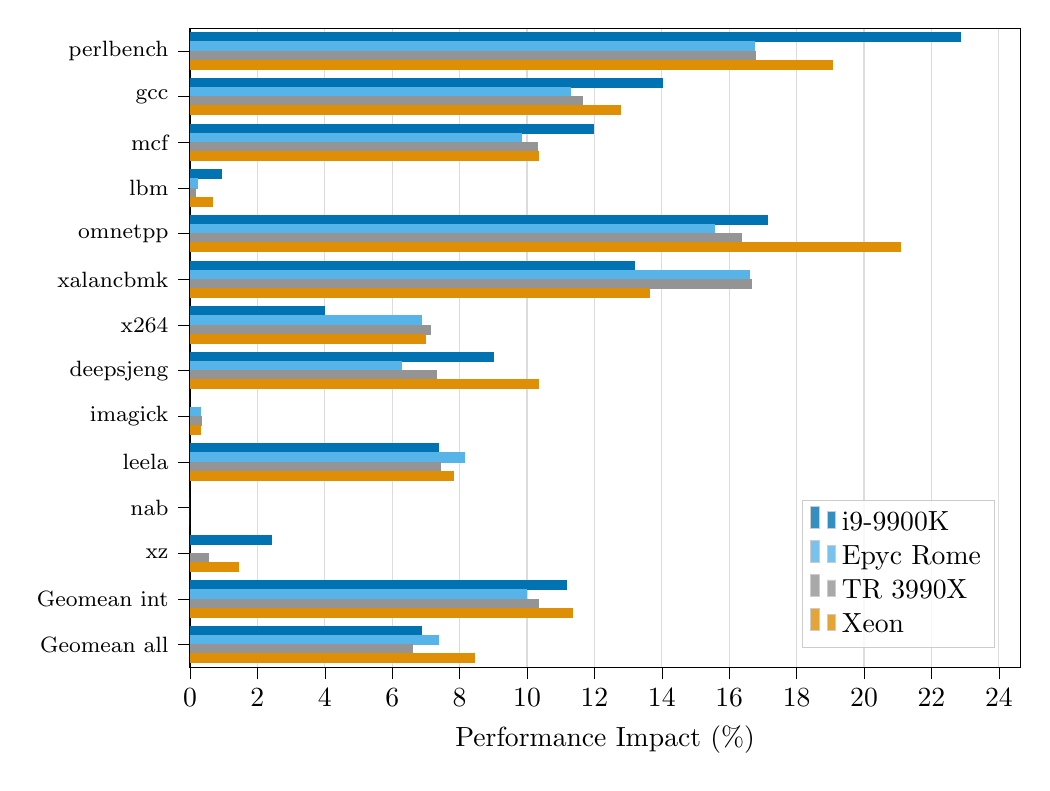
\begin{tikzpicture}

\definecolor{cornflowerblue86180233}{RGB}{86,180,233}
\definecolor{darkcyan1115178}{RGB}{1,115,178}
\definecolor{darkgray176}{RGB}{176,176,176}
\definecolor{darkorange2221435}{RGB}{222,143,5}
\definecolor{gainsboro}{RGB}{220,220,220}
\definecolor{lightgray204}{RGB}{204,204,204}
\definecolor{lightslategray148}{RGB}{148,148,148}

\begin{axis}[
legend cell align={left},
legend style={
  fill opacity=0.8,
  draw opacity=1,
  text opacity=1,
  at={(0.97,0.03)},
  anchor=south east,
  draw=lightgray204
},
tick align=outside,
tick pos=left,
x grid style={gainsboro},
xlabel={Performance Impact (\%)},
xmajorgrids,
xmin=0, xmax=24.6339961082686,
xminorgrids,
xtick style={color=black},
y dir=reverse,
y grid style={darkgray176},
ymin=-4.08, ymax=110.16,
ytick style={color=black},
ytick={0,8.16,16.32,24.48,32.64,40.8,48.96,57.12,65.28,73.44,81.6,89.76,97.92,106.08},
yticklabels={
  perlbench,
  gcc,
  mcf,
  lbm,
  omnetpp,
  xalancbmk,
  x264,
  deepsjeng,
  imagick,
  leela,
  nab,
  xz,
  Geomean int,
  Geomean all
}
]
\draw[draw=none,fill=darkcyan1115178,line width=0.32pt] (axis cs:0,-3.33) rectangle (axis cs:22.8868728825438,-1.53);
\addlegendimage{ybar,ybar legend,draw=none,fill=darkcyan1115178,line width=0.32pt}
\addlegendentry{i9-9900K}

\draw[draw=none,fill=cornflowerblue86180233,line width=0.32pt] (axis cs:0,-1.71) rectangle (axis cs:16.7569149267538,0.0900000000000001);
\addlegendimage{ybar,ybar legend,draw=none,fill=cornflowerblue86180233,line width=0.32pt}
\addlegendentry{Epyc Rome}

\draw[draw=none,fill=lightslategray148,line width=0.32pt] (axis cs:0,-0.0900000000000001) rectangle (axis cs:16.8038011920932,1.71);
\addlegendimage{ybar,ybar legend,draw=none,fill=lightslategray148,line width=0.32pt}
\addlegendentry{TR 3990X}

\draw[draw=none,fill=darkorange2221435,line width=0.32pt] (axis cs:0,1.53) rectangle (axis cs:19.0731603607468,3.33);
\addlegendimage{ybar,ybar legend,draw=none,fill=darkorange2221435,line width=0.32pt}
\addlegendentry{Xeon}

\draw[draw=none,fill=darkcyan1115178,line width=0.32pt] (axis cs:0,4.83) rectangle (axis cs:14.0450537040183,6.63);
\draw[draw=none,fill=cornflowerblue86180233,line width=0.32pt] (axis cs:0,6.45) rectangle (axis cs:11.2952207585287,8.25);
\draw[draw=none,fill=lightslategray148,line width=0.32pt] (axis cs:0,8.07) rectangle (axis cs:11.6585751865229,9.87);
\draw[draw=none,fill=darkorange2221435,line width=0.32pt] (axis cs:0,9.69) rectangle (axis cs:12.7996766901981,11.49);
\draw[draw=none,fill=darkcyan1115178,line width=0.32pt] (axis cs:0,12.99) rectangle (axis cs:11.9920579890501,14.79);
\draw[draw=none,fill=cornflowerblue86180233,line width=0.32pt] (axis cs:0,14.61) rectangle (axis cs:9.86311885819027,16.41);
\draw[draw=none,fill=lightslategray148,line width=0.32pt] (axis cs:0,16.23) rectangle (axis cs:10.3171873907563,18.03);
\draw[draw=none,fill=darkorange2221435,line width=0.32pt] (axis cs:0,17.85) rectangle (axis cs:10.3658053647033,19.65);
\draw[draw=none,fill=darkcyan1115178,line width=0.32pt] (axis cs:0,21.15) rectangle (axis cs:0.952682519924042,22.95);
\draw[draw=none,fill=cornflowerblue86180233,line width=0.32pt] (axis cs:0,22.77) rectangle (axis cs:0.227547204198286,24.57);
\draw[draw=none,fill=lightslategray148,line width=0.32pt] (axis cs:0,24.39) rectangle (axis cs:0.167724868513996,26.19);
\draw[draw=none,fill=darkorange2221435,line width=0.32pt] (axis cs:0,26.01) rectangle (axis cs:0.679115900161542,27.81);
\draw[draw=none,fill=darkcyan1115178,line width=0.32pt] (axis cs:0,29.31) rectangle (axis cs:17.1498282914226,31.11);
\draw[draw=none,fill=cornflowerblue86180233,line width=0.32pt] (axis cs:0,30.93) rectangle (axis cs:15.5682312732366,32.73);
\draw[draw=none,fill=lightslategray148,line width=0.32pt] (axis cs:0,32.55) rectangle (axis cs:16.3933840735117,34.35);
\draw[draw=none,fill=darkorange2221435,line width=0.32pt] (axis cs:0,34.17) rectangle (axis cs:21.0953074822708,35.97);
\draw[draw=none,fill=darkcyan1115178,line width=0.32pt] (axis cs:0,37.47) rectangle (axis cs:13.2106412464191,39.27);
\draw[draw=none,fill=cornflowerblue86180233,line width=0.32pt] (axis cs:0,39.09) rectangle (axis cs:16.6303425352307,40.89);
\draw[draw=none,fill=lightslategray148,line width=0.32pt] (axis cs:0,40.71) rectangle (axis cs:16.6827678304087,42.51);
\draw[draw=none,fill=darkorange2221435,line width=0.32pt] (axis cs:0,42.33) rectangle (axis cs:13.6502610201018,44.13);
\draw[draw=none,fill=darkcyan1115178,line width=0.32pt] (axis cs:0,45.63) rectangle (axis cs:4.0021259106342,47.43);
\draw[draw=none,fill=cornflowerblue86180233,line width=0.32pt] (axis cs:0,47.25) rectangle (axis cs:6.88269310214402,49.05);
\draw[draw=none,fill=lightslategray148,line width=0.32pt] (axis cs:0,48.87) rectangle (axis cs:7.15800878109507,50.67);
\draw[draw=none,fill=darkorange2221435,line width=0.32pt] (axis cs:0,50.49) rectangle (axis cs:6.99999430082181,52.29);
\draw[draw=none,fill=darkcyan1115178,line width=0.32pt] (axis cs:0,53.79) rectangle (axis cs:9.03135163641451,55.59);
\draw[draw=none,fill=cornflowerblue86180233,line width=0.32pt] (axis cs:0,55.41) rectangle (axis cs:6.30077796906123,57.21);
\draw[draw=none,fill=lightslategray148,line width=0.32pt] (axis cs:0,57.03) rectangle (axis cs:7.33675961216422,58.83);
\draw[draw=none,fill=darkorange2221435,line width=0.32pt] (axis cs:0,58.65) rectangle (axis cs:10.3637937448286,60.45);
\draw[draw=none,fill=darkcyan1115178,line width=0.32pt] (axis cs:0,61.95) rectangle (axis cs:-3.48273235558078,63.75);
\draw[draw=none,fill=cornflowerblue86180233,line width=0.32pt] (axis cs:0,63.57) rectangle (axis cs:0.327088091908423,65.37);
\draw[draw=none,fill=lightslategray148,line width=0.32pt] (axis cs:0,65.19) rectangle (axis cs:0.364197863129845,66.99);
\draw[draw=none,fill=darkorange2221435,line width=0.32pt] (axis cs:0,66.81) rectangle (axis cs:0.329224164470721,68.61);
\draw[draw=none,fill=darkcyan1115178,line width=0.32pt] (axis cs:0,70.11) rectangle (axis cs:7.38961334587653,71.91);
\draw[draw=none,fill=cornflowerblue86180233,line width=0.32pt] (axis cs:0,71.73) rectangle (axis cs:8.15781053170261,73.53);
\draw[draw=none,fill=lightslategray148,line width=0.32pt] (axis cs:0,73.35) rectangle (axis cs:7.44074750702926,75.15);
\draw[draw=none,fill=darkorange2221435,line width=0.32pt] (axis cs:0,74.97) rectangle (axis cs:7.84597997176371,76.77);
\draw[draw=none,fill=darkcyan1115178,line width=0.32pt] (axis cs:0,78.27) rectangle (axis cs:-12.0555916319535,80.07);
\draw[draw=none,fill=cornflowerblue86180233,line width=0.32pt] (axis cs:0,79.89) rectangle (axis cs:-0.62458622352014,81.69);
\draw[draw=none,fill=lightslategray148,line width=0.32pt] (axis cs:0,81.51) rectangle (axis cs:-11.5601370968125,83.31);
\draw[draw=none,fill=darkorange2221435,line width=0.32pt] (axis cs:0,83.13) rectangle (axis cs:-0.586622687852534,84.93);
\draw[draw=none,fill=darkcyan1115178,line width=0.32pt] (axis cs:0,86.43) rectangle (axis cs:2.44178427320745,88.23);
\draw[draw=none,fill=cornflowerblue86180233,line width=0.32pt] (axis cs:0,88.05) rectangle (axis cs:-0.379151137889988,89.85);
\draw[draw=none,fill=lightslategray148,line width=0.32pt] (axis cs:0,89.67) rectangle (axis cs:0.561134004435138,91.47);
\draw[draw=none,fill=darkorange2221435,line width=0.32pt] (axis cs:0,91.29) rectangle (axis cs:1.46630841417743,93.09);
\draw[draw=none,fill=darkcyan1115178,line width=0.32pt] (axis cs:0,94.59) rectangle (axis cs:11.1854352509048,96.39);
\draw[draw=none,fill=cornflowerblue86180233,line width=0.32pt] (axis cs:0,96.21) rectangle (axis cs:9.98814855472583,98.01);
\draw[draw=none,fill=lightslategray148,line width=0.32pt] (axis cs:0,97.83) rectangle (axis cs:10.3598398758856,99.63);
\draw[draw=none,fill=darkorange2221435,line width=0.32pt] (axis cs:0,99.45) rectangle (axis cs:11.3721724463311,101.25);
\draw[draw=none,fill=darkcyan1115178,line width=0.32pt] (axis cs:0,102.75) rectangle (axis cs:6.89240575278629,104.55);
\draw[draw=none,fill=cornflowerblue86180233,line width=0.32pt] (axis cs:0,104.37) rectangle (axis cs:7.39476375402615,106.17);
\draw[draw=none,fill=lightslategray148,line width=0.32pt] (axis cs:0,105.99) rectangle (axis cs:6.62388933065103,107.79);
\draw[draw=none,fill=darkorange2221435,line width=0.32pt] (axis cs:0,107.61) rectangle (axis cs:8.45098262457327,109.41);
\end{axis}

\end{tikzpicture}
}%
    \endgroup    \caption{The performance impact of full protection with \rtwoc on four different machines (see \cref{r2c:sss:full-overhead}).}
    % \propername{Geomean int} shows the geometric mean overhead of the SPEC CPU 2017 integer benchmarks only and \propername{geomean all} of the entire benchmark suite.}
    \label{r2c:fig:perf-full}
\end{figure}

We configured \rtwoc{} to insert between zero and five \glspl{heapbt} per function, but disabled other diversification measures.
\cref{r2c:fig:perf-components} shows that the geometric mean overhead of \glspl{heapbt} is 2\% with \propername{xalancbmk} causing the maximum overhead of 5\%.
The optimization to insert \glspl{heapbt} only in functions that write to their stack frame improves performance by 1\%.

\subsubsection{Prolog \& Layout Randomization}\label{r2c:sss:eval-layout}
We also isolated the performance impact of prolog trap insertion, and code- and data-layout randomization techniques---i.e., stack slot shuffling, global variable shuffling, and register-allocation randomization.
The prolog insertion randomly inserts between one and five traps into each function prolog, causing a geometric mean overhead of 2\%, with \propername{xalancbmk} being most affected at 6\%.
The combination of layout randomization techniques generally caused negligible overhead.

% \vspace*{-1em}

\subsubsection{Full \rtwoc}\label{r2c:sss:full-overhead}
We built a configuration with all \rtwoc{} protections enabled (see \cref{r2c:fig:perf-full}).
% would be nice to reiterate, but space is precious
This configuration
\begin{enumerate*}[label={(\roman*)}]
    \item protects return addresses with \glspl{BTRA} (see \cref{r2c:ss:impl-btras});
    \item injects \glspl{heapbt} (see \cref{r2c:ss:impl-heap-boobytraps});
    \item performs stack slot shuffling, global variable shuffling and register-allocation randomization;
    \item and inserts traps into function prologs and NOPs at call sites (see \cref{r2c:ss:strengthening}).
\end{enumerate*}
The geometric mean overhead is similar on all systems, with the \propername{Xeon} machine showing the highest overhead at 8.5\% for the full benchmark suite.
In \cref{r2c:fig:perf-components} the stacked bars (bars with differently colored sections) show the summed component overhead.
To contrast this artificially summed overhead with the actual overhead of all components working together, the dashed bars in \cref{r2c:fig:perf-components} show the real overhead for full \rtwoc on \propername{EPYC}.
For most benchmarks, the sum of component overheads accurately predicts the actual total overhead.
For \propername{mcf} and \propername{omnetpp}, however, the actual overhead is higher than the sum of components and for \propername{xalancbmk} it is lower.

Some benchmarks show diverging results on different machines.
On \propername{i9-9900K}, \propername{perlbench} has a significantly higher overhead than on the other machines.
For \propername{omnetpp}, the \propername{Xeon} machine has the highest overhead at 21\%.
Conversely, \propername{xalancbmk} shows better results on \propername{i9-9900K} and \propername{Xeon} than on the AMD machines.

On \propername{i9-9900K}, we found the webserver throughput \emph{decrease} to be 13\% for \propername{nginx} and 12\% for \propername{Apache}.
On the AMD machines, the throughput decrease was between 3 and 4 percent for both \propername{nginx} and \propername{Apache}.

%    \subsubsection{Adaptive parameter selection}\label{r2c:sss:adaptive}
%    To demonstrate the advantages of adaptive security, we built two configurations with adaptive parameter selection based on performance profiles.
%    Note that the performance profiles also influence LLVM's optimization decisions.
%    For that reason we compared the configurations with adaptive parameter selection to a (faster) profile-enabled baseline.
%    The configuration \propername{Adaptive-PR1} uses the parameter range $[0,2]$ for the lower bound, and the range $[2,5]$ for the upper bound of the subsequent random trial.
%    As a result, the random trial for the coolest call site samples from $[2,5]$ and for the hottest call sites from $[0,2]$ (see \cref{r2c:ss:impl-pgo} for the details).
%    The configuration \propername{Adaptive-PR2} provides better probabilistic security by using larger parameter ranges.
%    Specifically, \propername{Adaptive-PR2} uses a range of $[1,5]$ for the lower bound, and a range of $[2,10]$ for the upper bound.
%    The resulting random trial range for the coolest call sites is $[5,10]$ and for the hottest call sites $[1,2]$.
%    \propername{Adaptive-PR2} differs from \propername{Adaptive-PR1} by allowing twice as many BTRAs in the cold call sites, and protecting even hot call sites with at least \emph{two} BTRAs (also see~\Cref{r2c:fig:average-decoy-counts} for BTRA distribution).
%
%    \rtwoc's use of performance profiles positively influences performance in two ways.
%    First, performance profiles allow for more aggressive inlining:
%    Inlined call sites have no return address and, therefore, also do not need BTRAs.
%    Second, the profiles allow \rtwoc to decrease the number of BTRAs for hot call sites.
%    To evaluate these two effects separately, we built a configuration that uses a fixed number of ten BTRAs in total \emph{despite} the availability of performance profiles, thus cancelling out the effect of adaptive parameter selection.
%    From the comparison we can see that adaptive parameter selection still increases performance over the \propername{Fixed} configuration already optimized with inlining.


\subsubsection{Memory overhead}
To evaluate \rtwoc{}'s memory overhead we linked the benchmark programs from the SPEC CPU 2017 suite to a static library that prints the \propername{maxrss rusage} metric once the program ends.
The \propername{maxrss} metric is the maximum resident-set size of a process during its lifetime.
We chose this methodology because it allows measuring the memory overhead without impacting the benchmark performance.
With this methodology, we found the memory overhead of the SPEC benchmarks to be 1-3\%.

For the webserver benchmarks we had to choose a different methodology because the webservers spawn child processes.
With child processes, \propername{maxrss} reflects the maximum usage among all child processes instead of the combined maximum usage.
Instead, we started a separate monitoring process that records the RSS usage of each webserver process every second and calculated the median.
With this methodology, we found the memory overhead of the webserver benchmarks to be about 100\%.
We verified experimentally that about 55\% of the memory overhead is caused by the page allocations for \glspl{heapbt}.
The rest is caused by \glspl{BTRA} and the increased binary size.

\subsection{Scalability}\label{r2c:ss:scalability}
Although the SPEC benchmark suite covers a wide variety of test programs, we also compiled real-world software with \rtwoc.
Apart from Apache and nginx, we also compiled the GTK version of WebKit~\cite{Webkit} and Chromium~\cite{Chromium}.
We built both browsers with a fixed total number of 10 \glspl{BTRA} per call site.
WebKit and Chromium are massive \cpp projects with more than 4.5 million lines and almost 32 million lines of C/C\plusplus code, respectively.

To verify that \rtwoc does not introduce errors into the browser, we ran the included tests as well as the Speedometer browser benchmark.
To pass the tests, we had to modify a single source file in Chromium, and three source files in Webkit to deactivate \rtwoc for a few functions.
In both cases, unprotected code called an \rtwoc compiled function with stack arguments.
An example is the following function signature from WebKit's \propername{WebCore} module:
\begin{minted}[breaklines]{cpp}
static void gbkCallbackEscape(const void* context, UConverterFromUnicodeArgs* fromUArgs, const UChar* codeUnits, int32_t length, UChar32 codePoint, UConverterCallbackReason reason, UErrorCode* error);
\end{minted}
WebKit registers this function as a callback in the ICU unicode library.
The function has more parameters than can be passed in registers and, thus, needs stack arguments.
Unless the ICU library is compiled with \rtwoc, the calling code does perform \cfs (see \cref{r2c:sss:stack-arguments}).
We discuss this implementation limitation in \cref{r2c:ss:abi-change}.
We did not include the Speedometer performance results in the performance evaluation since Speedometer's results showed a variation of more than 20\% even in the baseline.
In daily browsing we did not notice any difference.

%%% Local Variables:
%%% mode: latex
%%% TeX-master: "../eurosys22"
%%% End:
